\documentclass[12pt,letterpaper]{article}
\usepackage[utf8]{inputenc}
\usepackage[spanish]{babel}
\usepackage{graphicx}
\usepackage[left=2cm,right=2cm,top=2cm,bottom=2cm]{geometry}
\usepackage{graphicx} % figuras
% \usepackage{subfigure} % subfiguras
\usepackage{float} % para usar [H]
\usepackage{amsmath}
\usepackage{minted}
%\usepackage{txfonts}
\usepackage{stackrel} 
\usepackage{multirow}
\usepackage{enumerate} % enumerados
\renewcommand{\labelitemi}{$-$}
\renewcommand{\labelitemii}{$\cdot$}
% \author{}
% \title{Caratula}
\begin{document}

% Fancy Header and Footer
% \usepackage{fancyhdr}
% \pagestyle{fancy}
% \cfoot{}
% \rfoot{\thepage}
%

% \usepackage[hidelinks]{hyperref} % CREA HYPERVINCULOS EN INDICE

% \author{}
\title{Caratula}

\begin{titlepage}
\begin{center}
\large{UNIVERSIDAD PRIVADA DE TACNA}\\
\vspace*{-0.025in}
\begin{figure}[htb]
\begin{center}

\includegraphics[width=8cm]{imagenes/logo.jpg}
\end{center}
\end{figure}
\vspace*{0.15in}
INGENIERIA DE SISTEMAS  \\

\vspace*{0.5in}
\begin{large}
TITULO:\\
\end{large}

\vspace*{0.1in}
\begin{Large}
\textbf{Trabajo Encargado Unidad II} \\
\end{Large}

\vspace*{0.3in}
\begin{Large}
\textbf{CURSO:} \\
\end{Large}

\vspace*{0.1in}
\begin{large}
INTELIGENCIA DE NEGOCIOS\\
\end{large}

\vspace*{0.3in}
\begin{Large}
\textbf{DOCENTE(ING):} \\
\end{Large}

\vspace*{0.1in}
\begin{large}
 Patrick Cuadros Quiroga\\
\end{large}

\vspace*{0.2in}
\vspace*{0.1in}
\begin{large}
Integrantes: \\
\begin{flushleft}
Moreno Mulluni Luis Angel		\hfill	(2017057864) \\
Layme Valeriano Diego 		\hfill	(2017057865) \\
Mamani Calisaya Yonathan 	           	\hfill	(2017057863) \\
\end{flushleft}
\end{large}
\end{center}

\end{titlepage}


\tableofcontents % INDICE
\thispagestyle{empty} % INDICE SIN NUMERO
\newpage
\setcounter{page}{1} % REINICIAR CONTADOR DE PAGINAS DESPUES DEL INDICE DE CUESTIONARIO

\section{Introducción}
\paragraph Both data and data warehouses are widely used to store big data, but there are no interchangeable terms. A data lake is an immense set of raw data. A data warehouse is a repository of filtered and structured data that has already been processed for a specific purpose.

People often confuse these types of data storage, when in fact they are greater than their similarities. In fact, the only real similarity between the two is its maximum purpose, which is to store data.

The difference is important, because they are designed for the objectives and the results. While it is better for a company to have a data lake, to obtain more results in the opportunity of a data warehouse.

\section{Resumen}
Tanto los datos como los almacenes de datos se utilizan de forma generalizada para almacenar big data, pero no hay términos intercambiables. Un lago de datos es un conjunto inmenso de datos en bruto. Un almacén de datos es un repositorio de datos filtrados y estructurados que ya han sido procesados ​​para una finalidad concreta.

La gente suele confundir estos tipos de almacenamiento de datos, cuando en realidad son mayores que sus semejanzas. A decir verdad, la única semejanza real entre ambos es su máxima finalidad, que es almacenar datos.

La diferencia es importante, porque están pensadas para los objetivos y los resultados. Mientras que a una empresa le conviene más tener un lago de datos, para obtener más resultados en la oportunidad de un almacén de datos.
\section{Materiales y Metodos}
    
    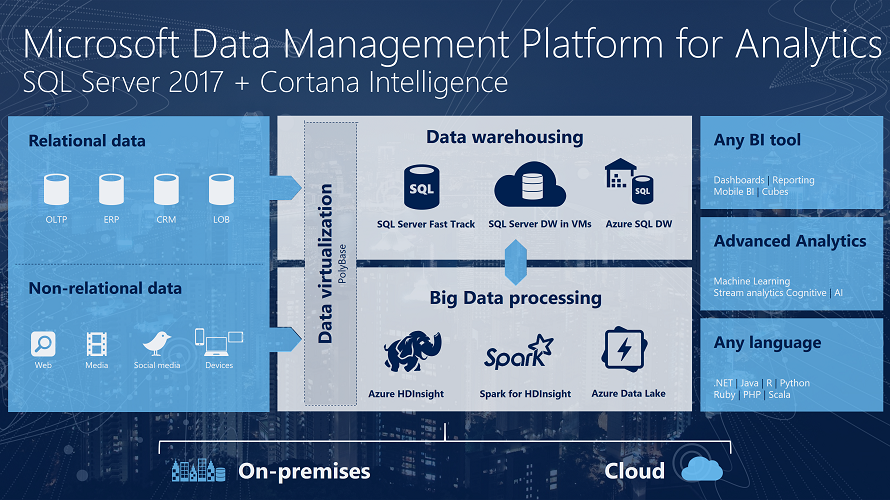
\includegraphics[width=16cm]{imagenes/arquitectura.png}
    
    \begin{enumerate}
        \item \textbf{¿ Por que necesitamos DataLake?}
        \paragraph Las organizaciones que generan valor de negocio exitosamente a partir de sus datos, superarán a sus pares. En una encuesta de Aberdeen, las organizaciones que implementaron un Data Lake superaron a las empresas similares en un 9 porciente en el crecimiento de ingresos orgánicos.\\ \\
        Estos líderes pudieron realizar nuevos tipos de análisis, como el aprendizaje automático a través de nuevas fuentes, como archivos de registro, datos de secuencias de clics, medios sociales y dispositivos conectados a Internet almacenados en el lago de datos. Esto les ayudó a identificar y aprovechar las oportunidades para el crecimiento empresarial más rápido al atraer y retener clientes, aumentar la productividad, mantener dispositivos de forma proactiva y tomar decisiones informadas.\\
        
        \item \textbf{Data Lakes comparado con Data Warehouses: dos enfoques diferentes}
        
        \paragraph Dependiendo de los requisitos, una organización típica requerirá tanto un almacén de datos como un lago de datos, ya que responden a diferentes necesidades y casos de uso.
        \paragraph Un almacén de datos es una base de datos optimizada para analizar datos relacionales provenientes de sistemas transaccionales y aplicaciones de línea de negocios. La estructura de datos y el esquema se definen de antemano para optimizar las consultas SQL rápidas, donde los resultados se utilizan normalmente para informes y análisis operativos. Los datos se limpian, enriquecen y transforman para que puedan actuar como la "fuente única de verdad" en la que los usuarios pueden confiar.
        
    \end{enumerate}

\section{Resultados}
    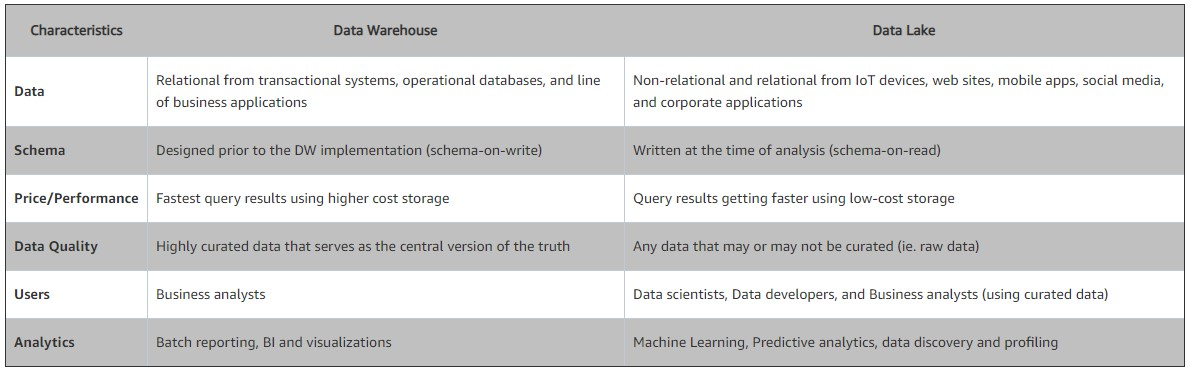
\includegraphics[width=17cm]{imagenes/cuadro_comparativo.jpg}
\section{Discusión}

    \begin{enumerate}
        \item \textbf{Data lakes frente a almacenes de datos: ¿Cuál me conviene más?}
        
        \paragraph Las organizaciones suelen necesitar ambos. Los data lakes se crearon por la necesidad de sacar partido a big data y aprovechar los datos estructurados y no estructurados granulados sin procesar para el machine learning, pero sigue existiendo la necesidad de crear almacenes de datos para que los usuarios corporativos les den una aplicación analítica.
        
        \item \textbf{Sanidad: Los data lakes guardan información no estructurada}
        \paragraph{Los almacenes de datos llevan años utilizándose en el sector de la sanidad, pero jamás se han cosechado grandes éxitos. Debido a la naturaleza no estructurada de gran parte de los datos del sector sanitario (notas de facultativos, datos clínicos, etc.) y a la necesidad de obtener información útil en tiempo real, los almacenes de datos no suelen ser un modelo idóneo.

Los data lakes permiten una combinación de datos estructurados y no estructurados, lo que en general encaja mejor para las empresas de este sector.}
        
        \item \textbf{Educación: Los data lakes ofrecen soluciones flexibles}
        
        \paragraph{Los últimos años se ha puesto de manifiesto a todas luces el valor de big data en las reformas educativas. Los datos sobre las calificaciones de los alumnos, asistencia, etc., no solo pueden ayudar a los alumnos en apuros a volver a encauzar sus estudios, sino que pueden contribuir a predecir posibles problemas antes de que ocurran. Las soluciones flexibles de big data también han ayudado a los centro educativos a racionalizar su facturación, mejorar la recaudación de fondos y en muchos otros frentes.

Gran parte de estos datos son extensos y se encuentran totalmente sin procesar, de modo que a menudo a los centros de enseñanza les conviene más la flexibilidad de los data lakes.}
        
        \item \textbf{Finanzas: Los almacenes de datos atraen a las masas}
        \paragraph{En las finanzas, como en otros entornos de negocios, un almacén de datos suele ser el mejor modelo de almacenamiento, porque puede estructurarse de forma que toda la empresa tenga acceso y no estrictamente los científicos de datos.

Big data ha permitido que el sector de los servicios financieros dé pasos agigantados, y los almacenes de datos han tenido mucho que ver a ese progreso. El único motivo por el que una empresa de servicios financieros decida optar por otro modelo es porque, si bien resulta más rentable, no es tan eficaz para otras finalidades.}
        
        \item \textbf{Transporte: Los data lakes ayudan a realizar predicciones}
        
        \paragraph{La gran ventaja de la información que aporta un data lake pasa por la capacidad de realizar predicciones.

En el sector del transporte, en especial en la gestión de la cadena de suministros, la capacidad predictiva que surge de los datos flexibles en un data lake puede tener grandes ventajas, a saber, la posibilidad de rebajar los precios que aporta el análisis de los datos de formularios de la canalización de transporte.}

        
    \end{enumerate}
\section{Conclusiones}
\paragraph El debate entre "data lakes o almacenes de datos" acaba de empezar, probablemente, pero las principales diferencias en estructura, procesamiento, usuarios y agilidad general hacen que cada modelo sea único. Según cuáles sean las necesidades de su empresa, resultará fundamental para su crecimiento crear el data lake o el almacén de datos más adecuado.

\begin{thebibliography}{9}
    \bibitem{talend} 
    Data lakes frente a almacenes de datos
    \textit{https://es.talend.com/resources/data-lake-vs-data-warehouse/}. 
    
    \bibitem{talend} 
    Data Lakes: Purposes, Practices, Patterns, and Platforms
    
    \bibitem{amazon} 
    What is a data lake?\\
    \textit{https://aws.amazon.com/es/big-data/datalakes-and-analytics/what-is-a-data-lake/}
    
    \bibitem{dbtest} 
    MICROSOFT DATA WAREHOUSE SOLUTIONS\\
    \textit{https://www.dbbest.com/technologies/azure-sql-data-warehouse/}
    
    \bibitem{PowerData} 
    Data Lake.
Superando las limitaciones
del Data Warehouse
    
    
    
    
    
    
    


\end{thebibliography}




\end{document}